\chapter[Improving Deep Neural Networks]{Improving Deep Neural Networks\setcounter{footnote}{0}\footnote{Hyperparameter Tuning, Regularization and Optimization}}

%%%
\section{Setting up and Regularizing neural network}

%%%%
\subsection{Train/dev/test sets}
对于数据集,我们通常将其分为三个部分:
\begin{itemize}
    \item \textbf{Training set}: 训练集,用于训练模型。一般占60\%。
    \item \textbf{Dev (development) set}: 开发集,用于调整模型的超参数。一般占20\%。
    \item \textbf{Test set}: 测试集,用于测试模型的性能。一般占20\%。
\end{itemize}
有时候,我们会将数据集仅分为训练集和开发集,而没有测试集。这时候,我们通常将二者的比例调整为70\%和30\%。

%%%%
\subsection{Bias and Variance}
\textbf{偏差(Bias)}描述了模型的预测值与真实值之间的差距。Bias越大,说明模型越不准确。
而\textbf{方差(Variance)}描述了模型的预测值与真实值之间的差距的方差。Variance越大,说明模型越不稳定。

\begin{figure}[h!bt]
    \centering
    \subfigure[High Bias]{
        \begin{minipage}[t]{0.3\textwidth}
            \centering
            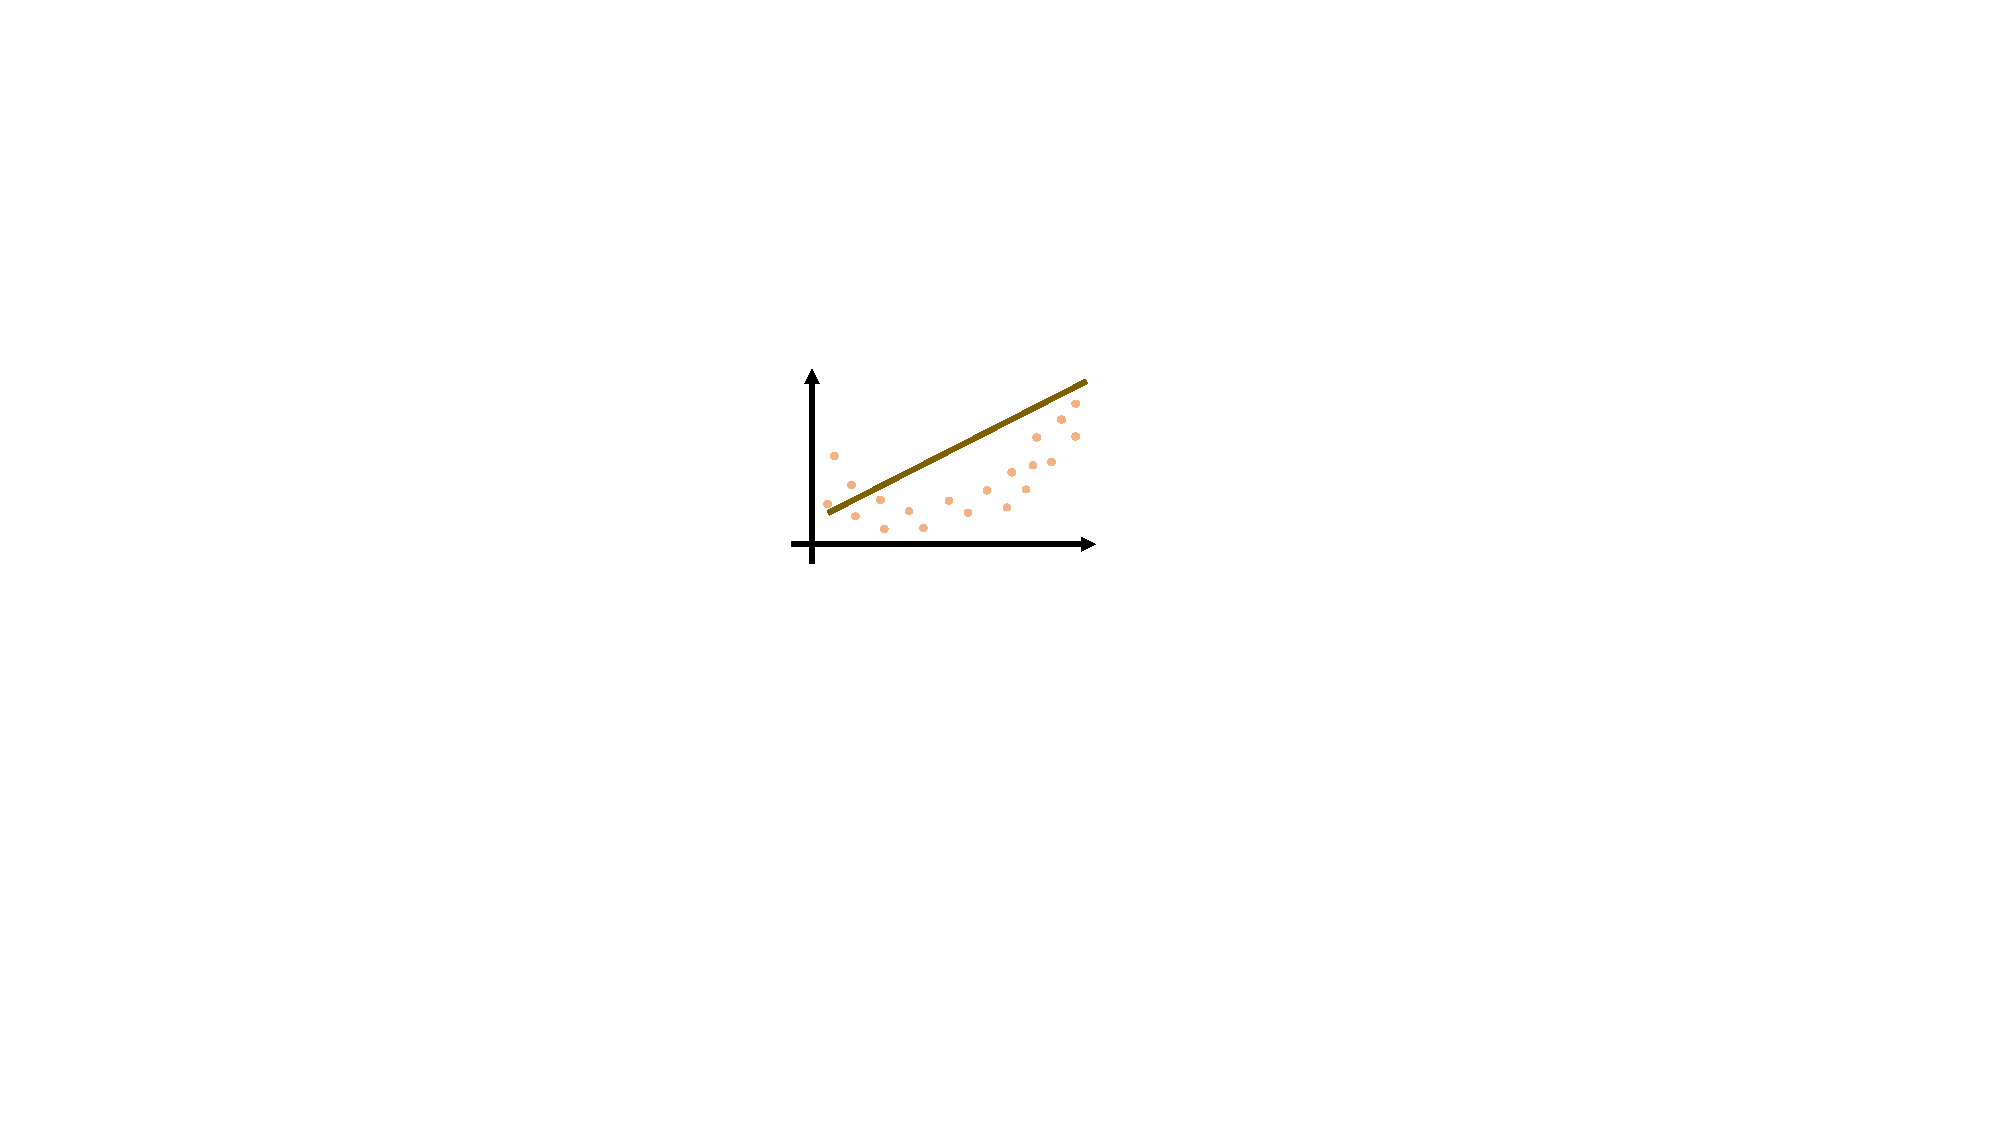
\includegraphics[scale=0.75]{high_bias.pdf}
        \end{minipage}
    }%
    \subfigure[Just Right]{
        \begin{minipage}[t]{0.3\textwidth}
            \centering
            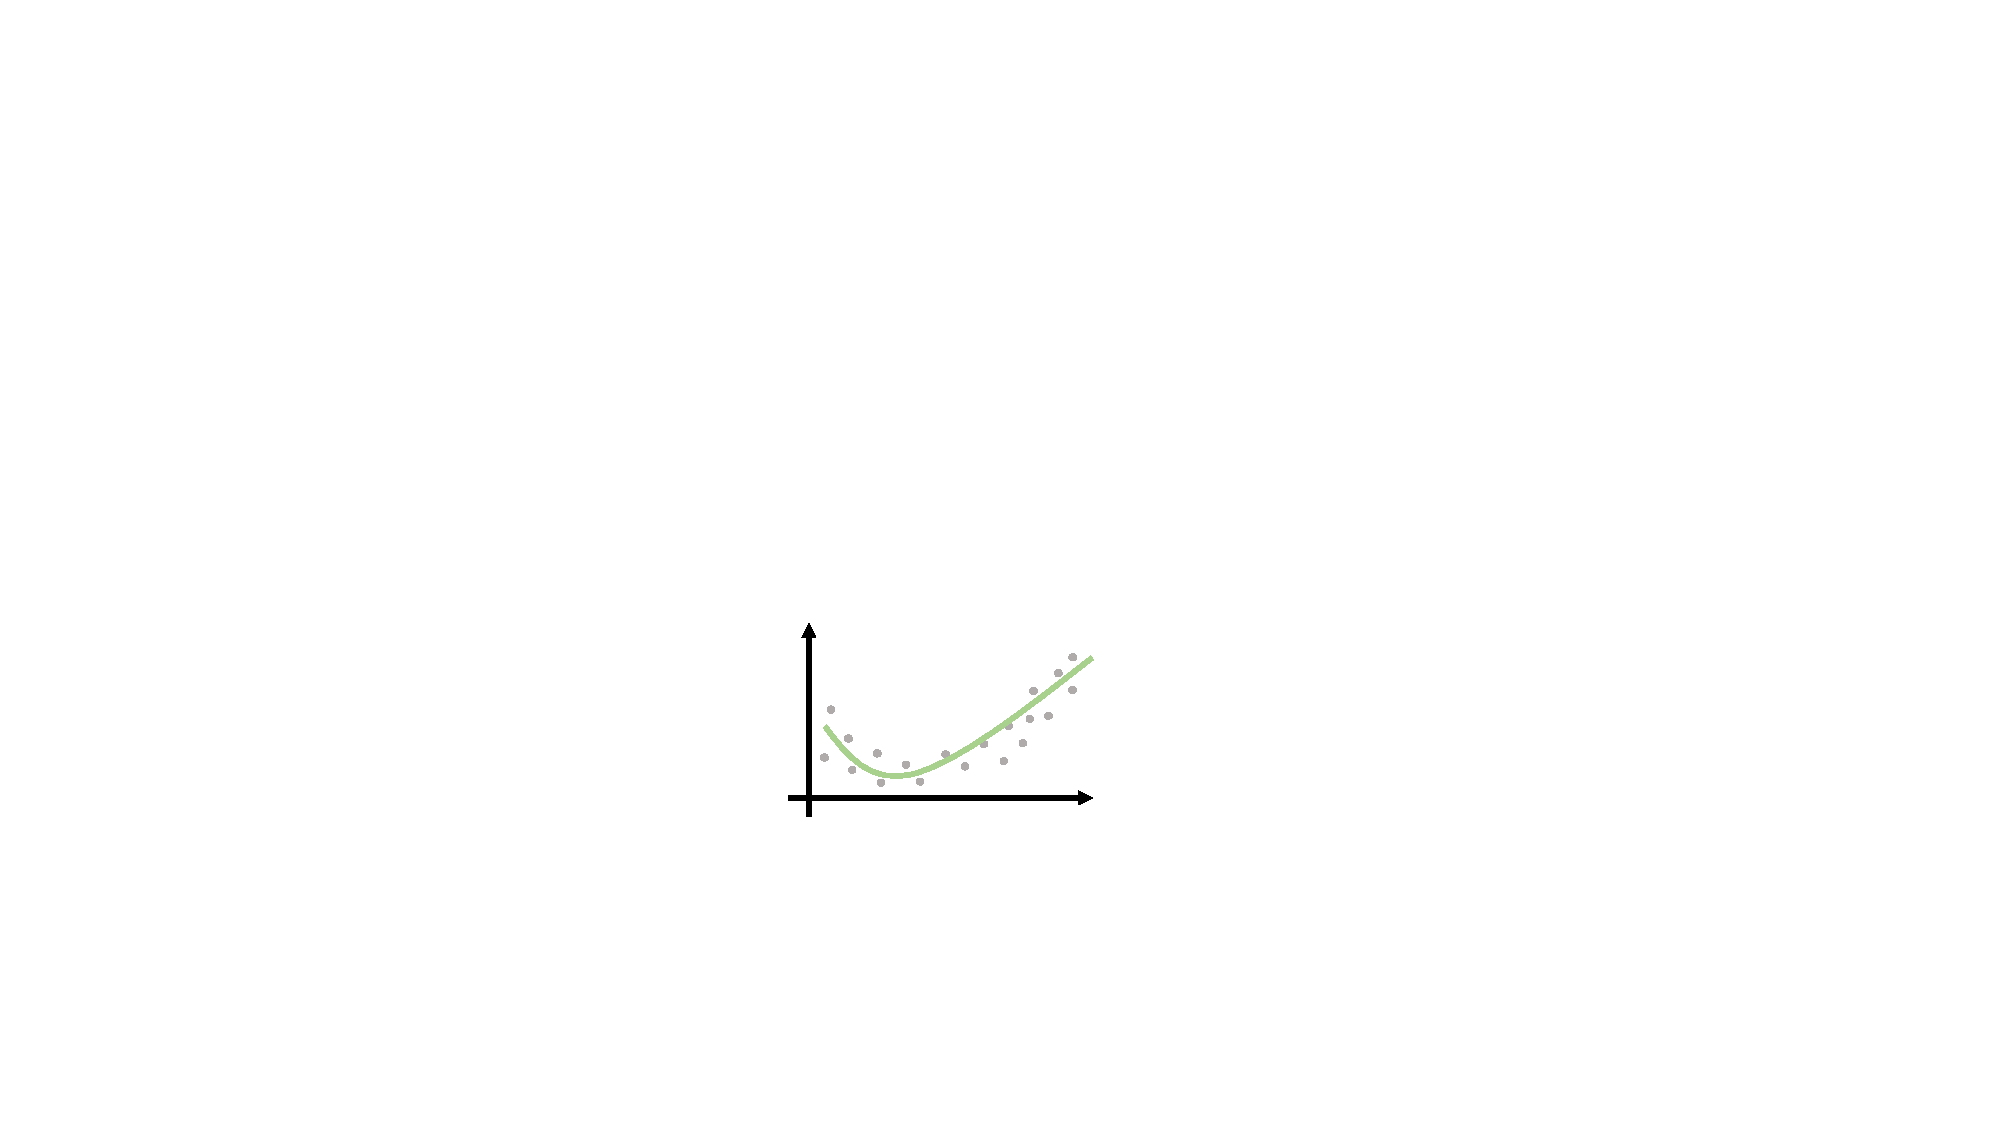
\includegraphics[scale=0.75]{just_right.pdf}
        \end{minipage}
    }%
    \subfigure[High Variance]{
        \begin{minipage}[t]{0.3\textwidth}
            \centering
            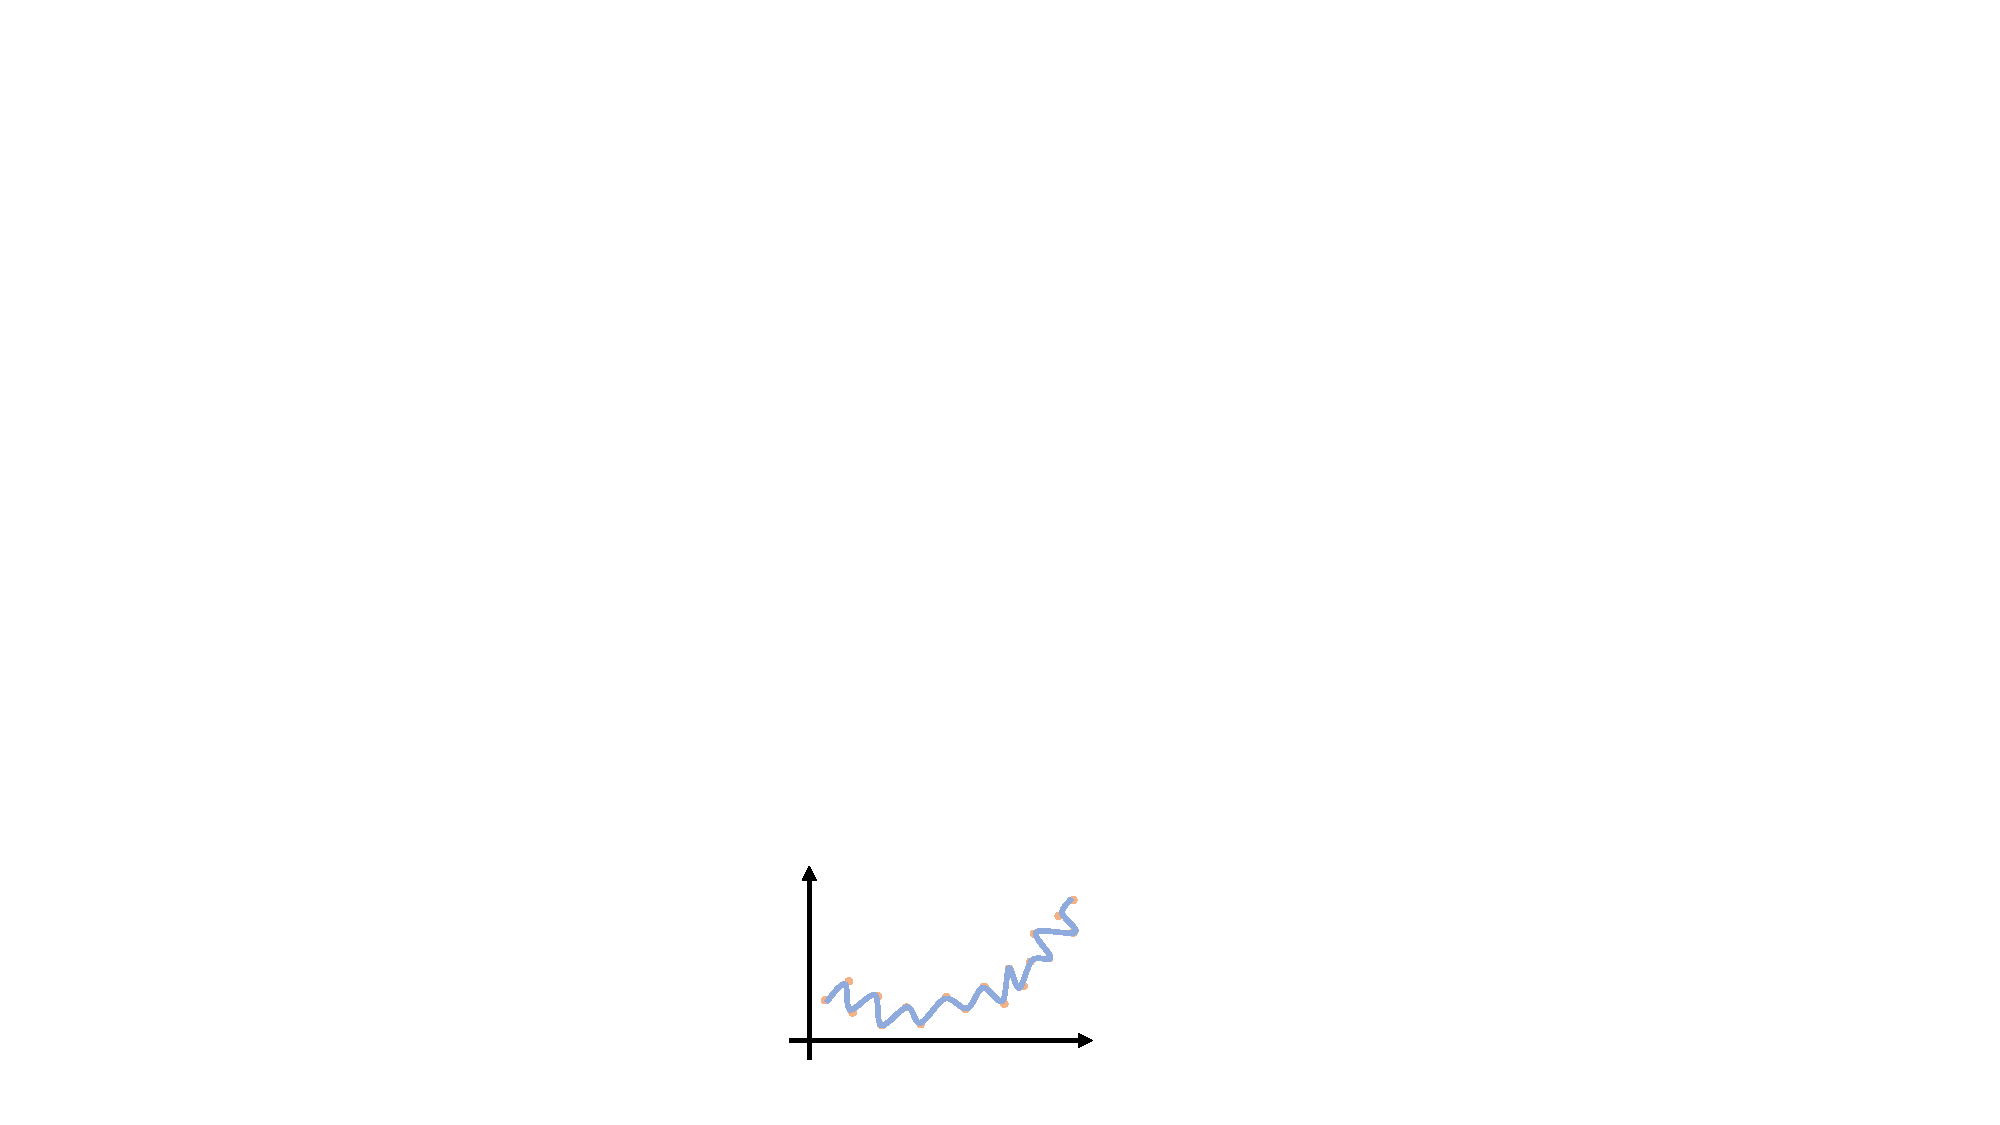
\includegraphics[scale=0.75]{high_variance.pdf}
        \end{minipage}
    }%
    \centering
    \caption{Bias and Variance}
    \label{fig:bias-variance}
\end{figure}

\textbf{高偏差(High bias)}通常表示模型欠拟合,即模型的复杂度不够,无法拟合数据。这可以体现在模型在训练集上的误差和在开发集上的误差都很大,且二者之间的差距不大。
而\textbf{高方差(High variance)}通常表示模型过拟合,即模型的复杂度过高,导致模型过于敏感,无法泛化。这可以体现在模型在训练集上的误差很小,但在开发集上的误差很大。
若高偏差和高方差同时存在,则会体现在模型在训练集上的误差和在开发集上的误差都很大,且开发集上的误差明显大于训练集上的误差。

当我们发现模型的偏差很大时,可以尝试使用更大的网络、训练更长的时间、使用更好的优化算法等来提高模型的复杂度,从而减小偏差。
而当我们发现模型的方差很大时,可以尝试使用更多的数据、使用正则化、使用dropout等来减小模型的复杂度,从而减小方差。

%%%%
\subsection{Regularization}
\index{Regularization}

正则化(Regularization)是一种减小模型复杂度的方法,可以防止模型过拟合。
正则化的方法有很多,这里介绍两种常用的正则化方法:$L_2$正则化和Dropout。

\begin{hint}
    正则化的目的是改变(通常是缩小)在更新权重和偏置时的梯度值,其本身并不干预模型的前向传播和反向传播过程。
\end{hint}

\subsubsection{$\mathsf{L_2}$ regularization}

$L_2$正则化($L_2$ regularization)也称为权重衰减(Weight Decay),是一种常用的正则化方法。
$L_2$正则化通过在代价函数中添加一个权重
\footnote{一般不对偏置做$L_2$正则化,避免影响神经元的激活阈值。}
的$L_2$范数
\footnote{$L_2$范数是针对向量的,而Frobenius范数是针对矩阵的,在这里并没有做严谨的区分。}
惩罚项来实现,这个惩罚项模型权重的平方成正比。这样做的目的是鼓励模型使用较小的权重,从而减少模型的复杂度。

$L_2$范数的定义是,对于一个长度为$n$的向量$w$,其$L_2$范数为:
\begin{equation}
    ||w||_2 = \sqrt{\sum_{j=1}^nw_j^2}
\end{equation}

使用$L_2$正则化后,代价函数中添加了各层权重信息的Frobenius范数,其计算公式为:
\begin{equation}
    J = \frac{1}{m}\sum_{i=1}^mL(\hat{y}^{(i)}, y^{(i)}) + \frac{\lambda}{2m}\sum_{l=1}^L||W^{[l]}||_{\mathrm{F}}^2
\end{equation}
其中$\lambda$为正则化参数,用于控制正则化的强度。$||W^{[l]}||_2^2$表示第$l$层权重Frobenius范数的平方,即
\begin{equation}
    ||W^{[l]}||_{\mathrm{F}}^2 = \sum_{i=1}^{n^{[l]}}\sum_{j=1}^{n^{[l-1]}}(W_{ij}^{[l]})^2
\end{equation}
添加这个惩罚项后,代价函数对权重的梯度为:
\begin{equation}
    \frac{\d J}{\d W^{[l]}} = \frac{\d J}{\d Z^{[l]}} A^{[l-1] \mathrm{T}} + \frac{\lambda}{m}W^{[l]}
\end{equation}
其他的梯度表达式保持不变(证明略)。

\subsubsection{Dropout}
\index{Dropout}

Dropout是一种常用的正则化方法,可以防止模型过拟合。Dropout的基本思想是,在每次迭代中,随机地关闭一些神经元,从而减小模型的复杂度。
Dropout 是以层为单位来使用的,即在设定的某些 Dropout 层中,每次迭代时,以一定的概率关闭其中的神经元。

需要注意,“关闭”神经元并不是将神经元中的权重和偏置清零,而只是将其输出置零。

\begin{figure}[h!bt]
    \centering
    \subfigure[随机选取神经元]{
        \begin{minipage}[t]{0.48\textwidth}
            \centering
            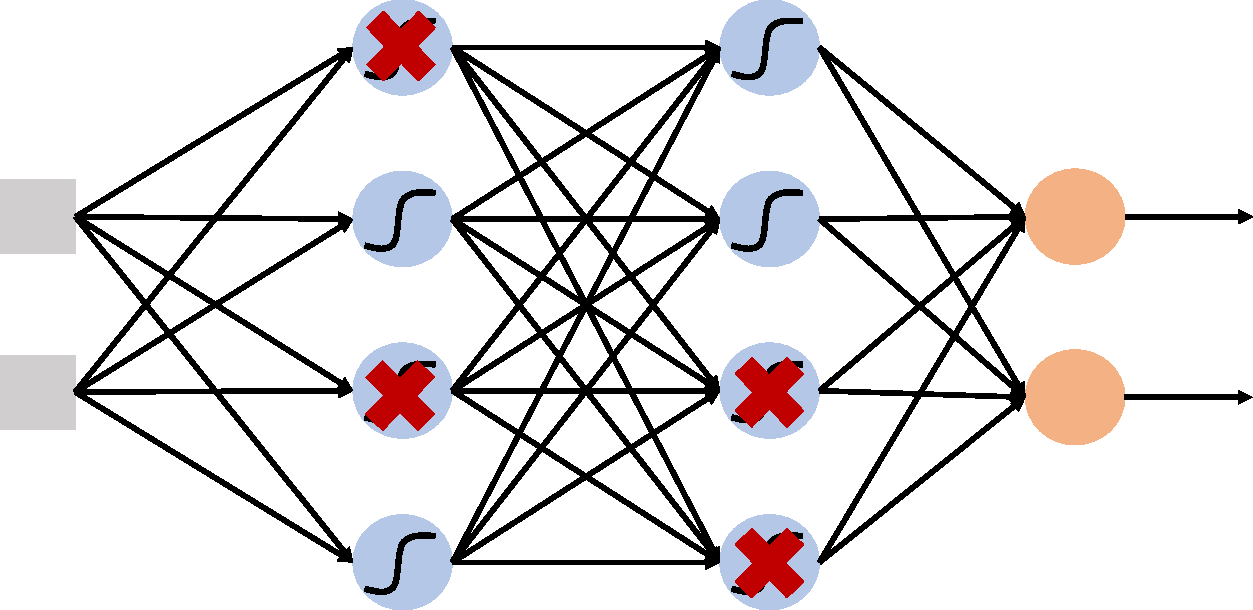
\includegraphics[width=0.8\textwidth]{dropout_1.pdf}
        \end{minipage}
    }%
    \subfigure[输出置零]{
        \begin{minipage}[t]{0.48\textwidth}
            \centering
            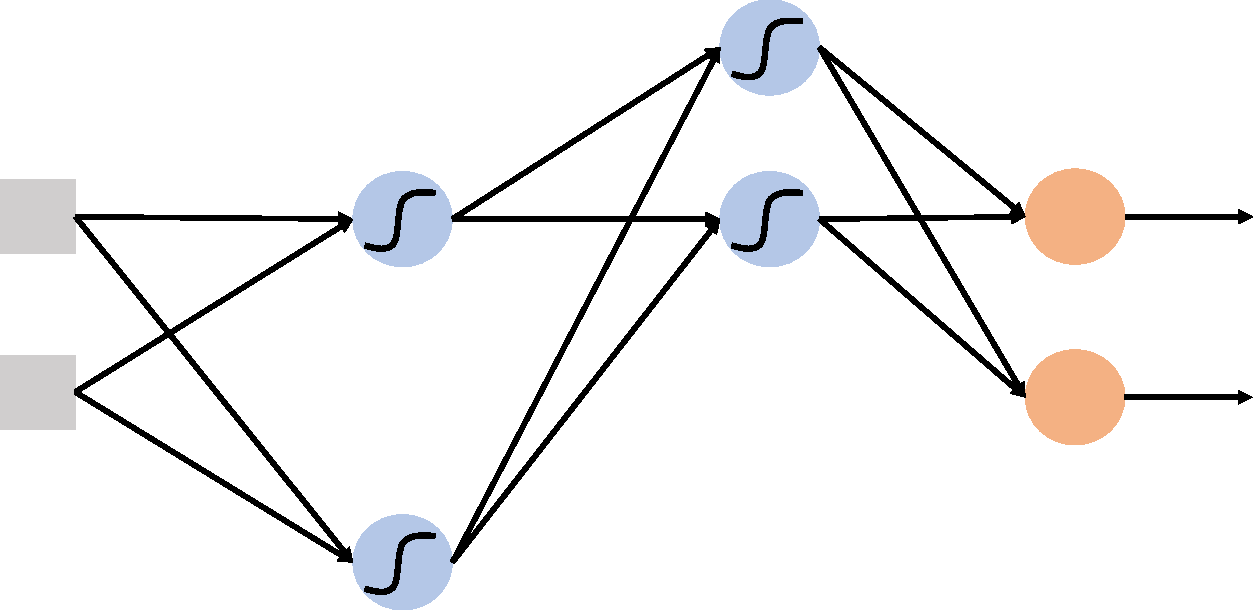
\includegraphics[width=0.8\textwidth]{dropout_2.pdf}
        \end{minipage}
    }%
    \centering
    \caption{Dropout}
    \label{fig:dropout}
\end{figure}

一种常见的Dropout实现为Inverted dropout。假设第$l$层被设置为Dropout层,设置一个保留概率 \verb|keep_prob| ,
则在每次迭代的前向传播中,先用原有的方式计算出第$l$层的激活值$A^{[l]}$,然后构造一个布尔矩阵
\begin{equation}
    \mathtt{D^{\textcolor{Magenta}{[}l\textcolor{Magenta}{]}}} = \mathtt{np.random.rand\textcolor{yellow}{(} A^{\textcolor{Magenta}{[}l\textcolor{Magenta}{]}}.shape\textcolor{Magenta}{[}\textcolor{green}{0}\textcolor{Magenta}{]}, A^{\textcolor{Magenta}{[}l\textcolor{Magenta}{]}}.shape\textcolor{Magenta}{[}\textcolor{green}{1}\textcolor{Magenta}{]} \textcolor{yellow}{)} < keep\_prob}
\end{equation}
将这个布尔矩阵与$A^{[l]}$相乘,即可将第$l$层的部分输出置零
\begin{equation}
    \mathtt{A^{\textcolor{Magenta}{[}l\textcolor{Magenta}{]}}} = \mathtt{np.multiply\textcolor{yellow}{(} A^{\textcolor{Magenta}{[}l\textcolor{Magenta}{]}}, D^{\textcolor{Magenta}{[}l\textcolor{Magenta}{]}} \textcolor{yellow}{)}}
\end{equation}
为了补偿训练过程中由于 Dropout 导致的输出值的减少,需要进行一次缩放,即
\begin{equation}
    \mathtt{A^{\textcolor{Magenta}{[}l\textcolor{Magenta}{]}}} /= \mathtt{keep\_prob}
\end{equation}
将这个值作为第$l$层的输出$A^{[l]}$。在反向传播中,使用这些经过 Dropout 的各层输出来计算梯度来更新权重和偏置。
从结果上看,这相当于这一轮迭代中的训练的神经元数“减少”了,可以降低模型对单个神经元的依赖,从而提高模型的泛化能力。

在评估模型或者使用模型进行预测时(此时只有前向传播),需要关闭Dropout。这是为了确保模型的输出与训练阶段保持一致,从而准确评估模型在未见数据上的性能。

\subsubsection{Other regularization methods}

除了$L_2$正则化和Dropout,还有一些其他的正则化方法,如数据增强(Data Augmentation)、早停(Early Stopping)等。

数据增强是一种简单有效的正则化方法,其基本思想是通过对训练集中的数据进行一些随机变换,从而生成更多的训练数据。
例如,对于图像分类问题,可以对图像进行一些随机的旋转、平移、缩放等操作,将其作为新增的训练数据。

早停的基本思想是在训练过程中,当模型在开发集上的误差连续一段时间不再下降时,就停止训练。
这样可以防止模型过拟合,但需要注意的是,早停的效果很大程度上依赖于开发集的选择。

\subsection{Normalizing Inputs}

在训练神经网络时,我们通常会对输入数据进行归一化处理。
归一化可以确保数值在可接受的范围内,将所有特征重现在相同的尺度上,提高算法的数值稳定性。

数据归一化通常包括两个步骤:减去平均值(使得归一化后的数据具有零均值)和除以标准差(使得归一化后的数据具有单位方差)。
这种方法也被称为 Z-score 标准化或标准化。在标准化后,数据的均值为0,标准差为1。

\begin{figure}[h!bt]
    \centering
    \subfigure[Before Normalization]{
        \begin{minipage}[t]{0.48\textwidth}
            \centering
            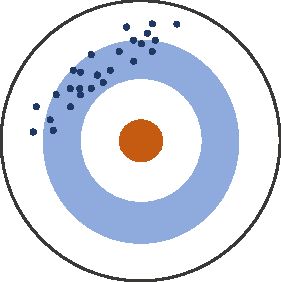
\includegraphics[scale=0.75]{norm_before.pdf}
        \end{minipage}
    }%
    \subfigure[After Normalization]{
        \begin{minipage}[t]{0.48\textwidth}
            \centering
            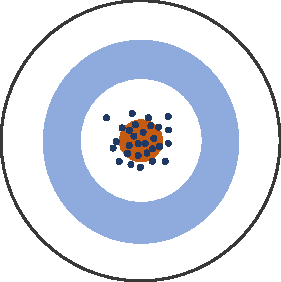
\includegraphics[scale=0.75]{norm_after.pdf}
        \end{minipage}
    }%
    \centering
    \caption{Normalization}
    \label{fig:normalization}
\end{figure}

在 python 中,可以很方便地实现输入数据的归一化
\begin{python}
X -= np.mean(X, axis=0)
X /= np.std(X, axis=0)
\end{python}

